\documentclass{article}

\usepackage[utf8]{inputenc}
\usepackage{graphicx}
\usepackage{caption}
\usepackage{subcaption}

\begin{document}
\section*{Introduction}
For the final project we were tasked to use what we have learned on a dataset of our choice. 
Since we both watch Youtube, we decided to work with a Youtube data set from the Kaggle collection. 
This dataset contains multiple sets of Youtube metadata from many countries around the world. 
Each country has the same columns but a wide variety of different Youtube videos and categories. 
In this project we focused on the USA data set since that had the most familiar videos. 
From the Youtube dataset our goal was to extract useful information about the trending videos; what videos are trending and how fast do they trend?
Using this information we wanted to use a decision tree to predict how long it will take for a video to go trending. 
There is a lot of information in these datasets that we are not using but would not aid the decision tree in its training or prediction.
Overall, it was interesting challenge for the decision tree algorithm to predict when a video will go trending.
\section*{Implementation}
%%TALK about exactly what our code is doing to achieve the goal

We want to build a decision tree to help us to predic the date based on our input data.
%
For decision tree, our input should be integer instead of text, so we can not input our data directly.
%
It means we need to preprocess our data into the right format.
%
At first, we choose these attributes that are helpful for our target. For attributes that are text formats we just convert them into category type because of the need of integer type input of decision tree.
%
And we have two different time in raw data attributes, we can summrize them by the duration.
%
Because our target is the time it takes from published time. So we can work out this duration and replace other dates.
%
There are also some data that might have some errors and they are already marked.
%
We also need to clean these data.
%
Then we split our data set into training and testing part.
%
We create a decision tree and input our train attribute data and target data to get a trained model.
%
After that we input our test data to see the accuracy of our decision tree.
%
In addition, we also add a tree for predicting the category of videos. It works much better.

\begin{figure}[!h]
    \centering
    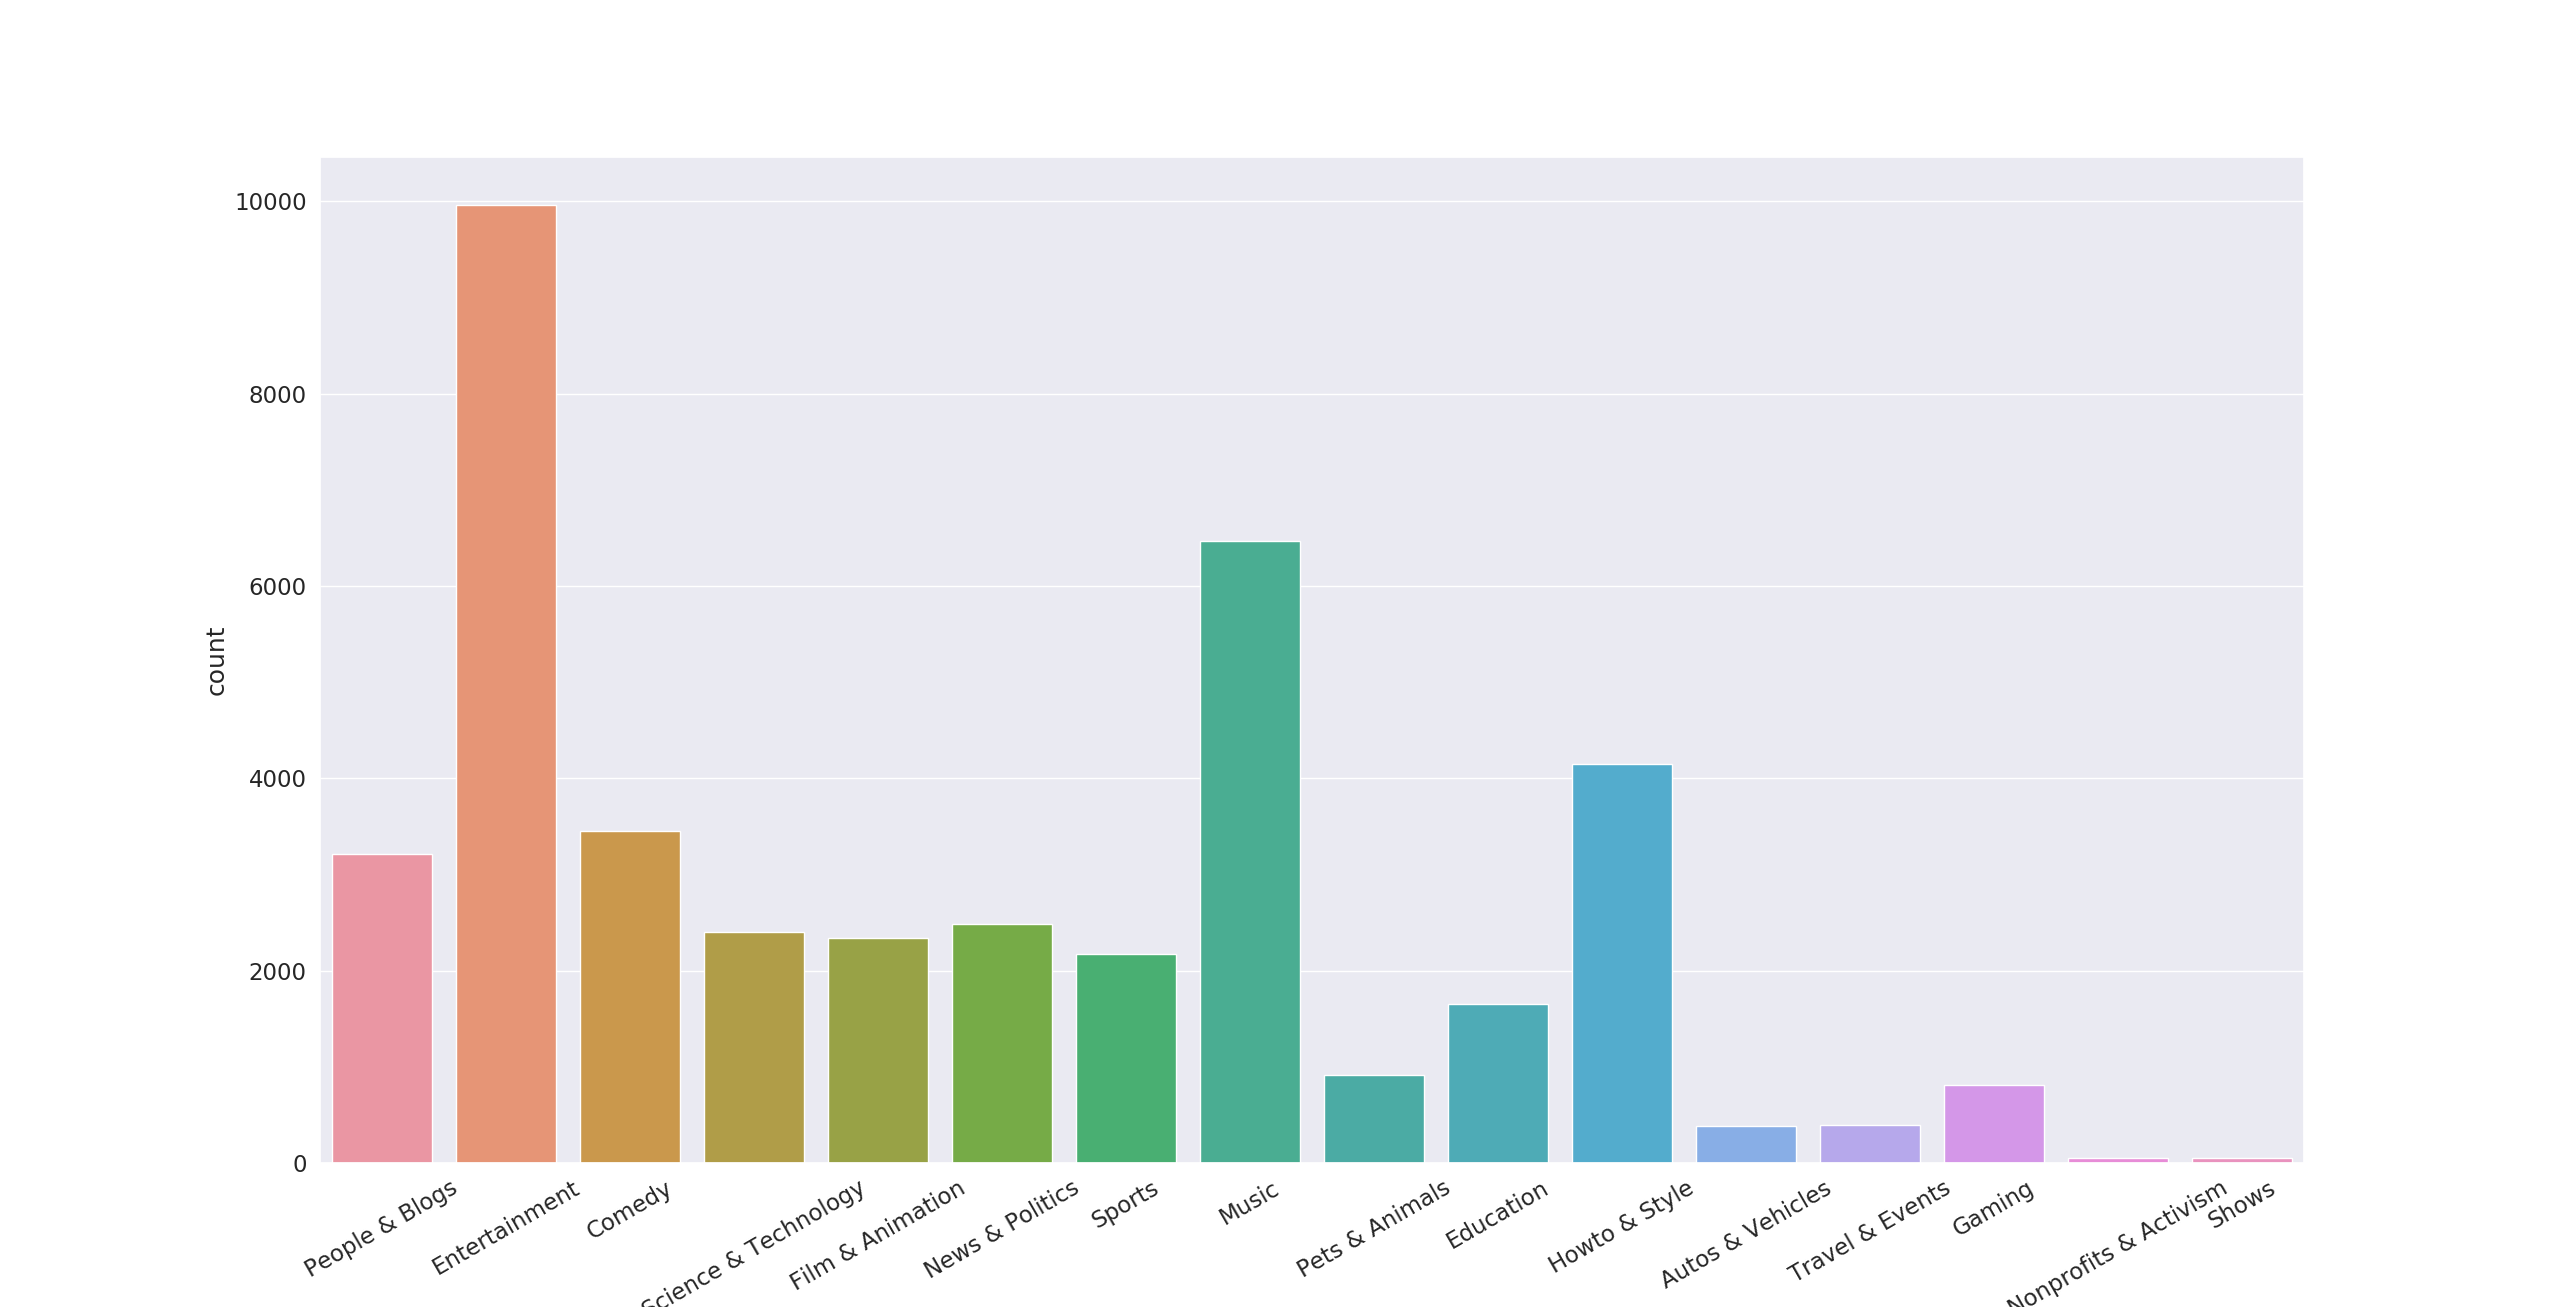
\includegraphics[width=1\textwidth]{category_graph.png}
    \caption{Amout of videos for each category}
    \label{fig:iris}
\end{figure}

\section*{Results}
\par
    After parsing our data and skimming it down to just the right columns, we still struggled to make the decision tree preform well.
We were barely even getting 10 percent accuracy from the tree.
Obviously, this not ideal and we ultimately would want the decision tree to preform well. 
This accuracy score is mostly due to the poor training data.
There just is not enough information and correlation between the data points used.
For example, if a video has 1,000,000 views but took 10 days to trend, then another video with the same amount videos only took 3 three days to trend, what was the difference between the two videos?
It can't be the likes or dislikes because you run into the same problem, so it must be something else. 
If you just go on YouTube and look at the current trending videos they all have crazy titles and thumbnails. 
These attributes likes images and text, cannot be used in a decision tree easily without the help of machine learning. 
The real reason our result is so low is because we use values that are ambiguous and don't have enough meaning to a specific video to label it as a category.
After rationalizing this, it makes complete sense.
We really wanted to test the absolute limit of what a decision tree could do.
For fun, we added some code that would create a decision tree for each category separately to see if we would get better results.
After doing this, and seeing all the numbers run down the screen, we quickly learned that we were achieving the same results as before.
Knowing that decision trees don't do well when then isn't an even distribution of the categories, we still wanted to see the outcome.
With this separation of the categories, there was still way too much variation in the data to have a good result. 
In the end, with all that we tried, a decision tree was not the best method for predicting when a video will be trending without parsing some textual data or using machine learning.

\par
    In an effort to make something work with the decision tree and our data, we attempted to predict the category of the video based on the metadata. 
This result was much more successful. We were averaging around 60 percent accuracy for which category was which. 
We still run into the same problem as before, where the numerical data doesn't fully represent each video.
But the prediction of the category is much easier.
It's not perfect, but our solution uses all of the relevant data to make it's prediction.
We can look at the category graph, thats inside the project and it shows the distribution of videos in a specific category. 
This shows how varied the number of videos are in each category. 
Since there is nothing consistent, our decision tree is doing its best to places the videos under a category.
We are getting better results because there is specific categories that the decision tree can pick and choose from.
Where the days of trending was such a wide range it was almost impossible for it to easily pick a specific time frame.
We were happy to see that we could do some prediction using the data. 
With our limitations we learned how far we could push the decision tree.

\section*{Conclusion}
    In conclusion, this was an ambitious goal, predicting how long will it take for a video to go trending. 
However, due to poor numerical data and difficult to work with textual data we were only able to get 10 percent accuracy. 
Working with numerical data is easy, but only if those numbers are solid and unambiguous. 
Working with textual is hard, and is still a researched project.
Even if we categorized the textual data (aside from the categories), we would be loosing a lot of information by doing so.
Knowing this now, if we wanted to improve our results, we would have to rely on machine learning to categorize or even predict videos based on there titles or thumbnails.
When I and on YouTube and looking at all the trending videos there is some consistency to which ones are at the top. 
And this is usually things like, is the video a music video, or does the YouTube video have tons of subscribers, or is the thumbnail super flashy. 
These are all factors that truly are the reason why a video goes trending.  
If you were able to use machine learning to capture and analyze, then you might be able to predict whether or not a video will trend for longer or shorter.
Finally, after doing some research, YouTube has its own algorithm that picks certain videos to be trending and how long. 
If you were to predict how long a video would be trending you would be learning exactly how the YouTube algorithm works. 
Then you could always make the most trending videos on YouTube. 
\end{document}
